%!TeX spellcheck = en-US
%!TEX root = ../hw4_report.tex

\subsection*{$(a)$}
Consider the approximate solution $X_{k} = V_{k}Y_{k}V_{k}^{T}$ for the Lyapunov equation
\begin{equation}
  AX+XA^{T} + BB^{T} = 0,
\end{equation}
where the columns of $V_{k}$ spans the subspace $K_{k}$ of $\mathbb{R}^{n}$. The columns are orthonormal. Furthermore, let $B = V_{K}E$ for some $E$. Introduce the residual
\begin{equation}
  R_{k} = AX_{k}+XA_{k}^{T} + BB^{T}
\end{equation}
and impose the it is orthogonal to $K$, i.e.
\begin{align}
  V_{k}^{T}R_{k}V_{k} = 0 &\Leftrightarrow V_{k}^{T}AV_{k}Y_{k}V_{k}^{T}V_{k}+V_{k}^{T}V_{k}Y_{k}V_{k}^{T}A_{k}^{T}V_{k} + EE^{T} = 0\\
  \label{eq:LyapY}
   &\Leftrightarrow V_{k}^{T}AV_{k}Y_{k}+Y_{k}V_{k}A^{T}V_{k}^{T} + EE^{T} = 0.
\end{align}
Introduce the short hand notation $H_{k} = V_{k}^{T}AV_{k}Y_{k}$ and a sequence of approximation spaces $K_{k}\subset K_{k+1}$ that satisfies $AK_{k}\subset K_{k+1}$. If $V_{k}$ spans $K_{k}$, then $K_{k+1}$ contains $AV_{k}$, which is spanned by the columns of $V_{k+1}$. Or in other words: $AV_{k}$ expressed in $K_{k+1}$ is $V_{k+1}\underline{H}_{k}$.
We can now rewrite the residual $R_{k}$ as
\begin{equation}
  R_{k} = V_{k}\underline{H}_{k}V_{k+1}^{T} X_{k}+XV_{k+1}^{T}\underline{H}_{k}^{T}V_{k} + V_{k}EE^{T}V_{k}^{T}.
\end{equation}


\subsection*{$(b)$}
From \eqref{eq:LyapY} we have that
\begin{equation*}
V_{k}^{T}AV_{k}Y_{k}+Y_{k}V_{k}A^{T}V_{k}^{T} + EE^{T} = 0,
\end{equation*}
and if $VYV^{T} = X$ is exact, then
\begin{equation*}
V^{T}AVY+YVA^{T}V^{T} + EE^{T} = 0.
\end{equation*}
Introduce $H_{k} = V_{k}^{T}AV_{k}$ and $H = V^{T}AV$. Then the approximate solutions $Y_{k}$ and
$X_{k}$ are given by
\begin{equation*}
Y_{k} =  \int\limits_{0}^{\infty}e^{tH_{k}}EE^{T}e^{{tH_{k}}^{T}}dt \Leftrightarrow V_{k}Y_{k}V_{k}^{T} =  \int\limits_{0}^{\infty}V_{k}e^{tH_{k}}EE^{T}e^{{tH_{k}}^{T}}V_{k}^{T}dt = X_{k}.
\end{equation*}
The analytical solution $X$ satisfies
\begin{equation*}
X =  \int\limits_{0}^{\infty}e^{tA}BB^{T}e^{{tA}^{T}}dt.
\end{equation*}
We know that $X = V_{k}Y_{k}V_{k}^{T}$, thus $H = H_{k} = V_{k}^{T}AV_{k}$ as well. With $B = V_{k}E$ we have
\begin{align*}
X &=  \int\limits_{0}^{\infty}e^{tA}BB^{T}e^{{tA}^{T}}dt =
\int\limits_{0}^{\infty}e^{tV_{k}HV_{k}^{T}}V_{k}EE^{T}V_{k}^{T}e^{tV_{k}H^{T}V_{k}^{T}}dt = \int\limits_{0}^{\infty}V_{k}e^{tH}V_{k}^{T}V_{k}EE^{T}V_{k}^{T}V_{k}e^{{tH}^{T}}V_{k}^{T}dt\\
&=\int\limits_{0}^{\infty}V_{k}e^{tH}EE^{T}e^{{tH}^{T}}V_{k}^{T}dt = X_{k}.
\end{align*}
That $e^{tV_{k}HV_{k}^{T}} = V_{k}e^{tH}V_{k}^{T}$ is a simple consequence of $V_{k}$ being orthonormal. By interpreting $e^{tV_{k}HV_{k}^{T}}$ via the Taylor series definition the matrices  $V_{k}$ and $V_{k}^{T}$ will cancel out. We have
\begin{align*}
  e^{tV_{k}HV_{k}^{T}} = \sum\limits_{i = 0}^{\infty}\frac{t^{i}}{i!}(V_{k}HV_{k}^{T})^{i}=V_{k}\left(\sum\limits_{i = 0}^{\infty}\frac{t^{i}}{i!}H^{i}\right)V_{k}^{T} = V_{k}e^{tH}V_{k}^{T}.
\end{align*}


\subsection*{$(c)$}
The claim that the singular values of positive, or negative, definite matrices converge faster than for indefinite matrices is supported in Figure \ref{13c}.
\begin{figure}[h!]
\centering
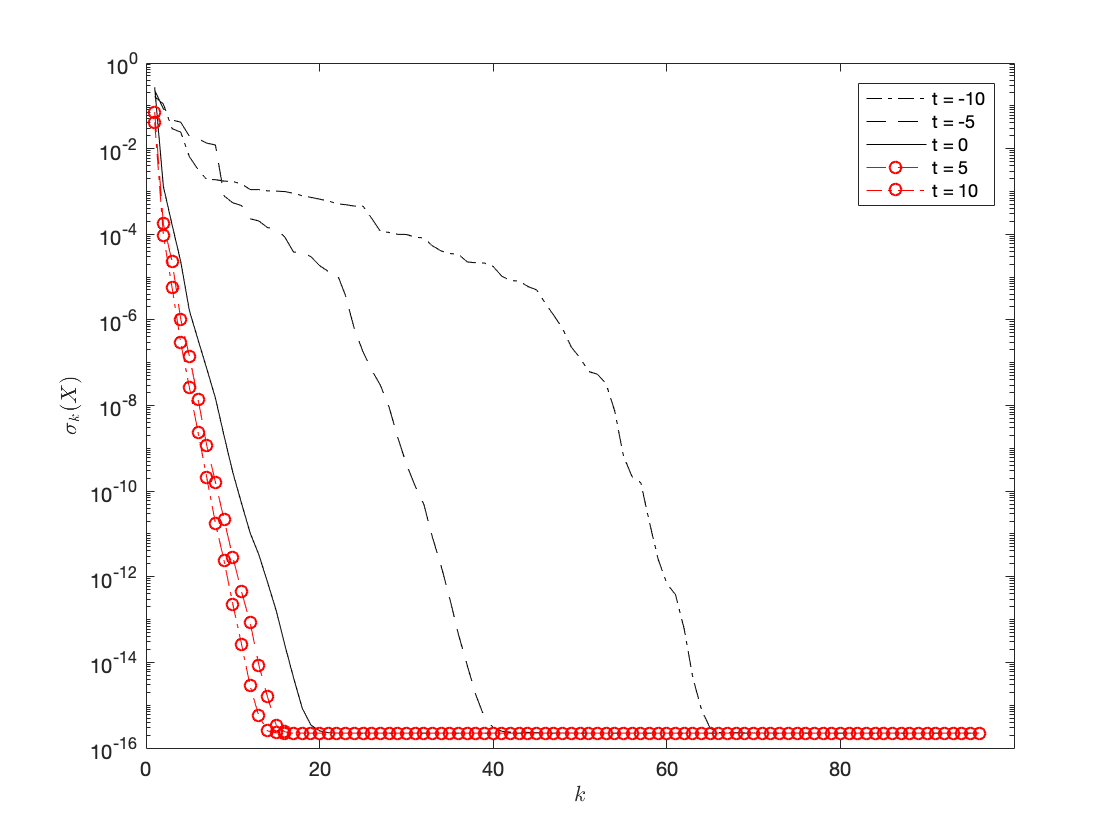
\includegraphics[scale=0.5]{task13c.png}
\caption{Task $13(c)$. }
\label{13c}
\end{figure}




\subsection*{$(d)$}
The largest problem I can solve on my machine is $nx = 167$ with \texttt{k-pik} and $nx = 17$ for \texttt{lyap}, for $t\in[0,1,10,100,1000]$. There is some small variation in $nx$ for \texttt{k-pik} with different $t$, but no more than $\pm 2$. For $nx = 17$  \texttt{lyap} gives an error about $1e-14$ for the given range of $t$. For \texttt{k-pik} $t=0$ and $t = 1$ the error is of magnitude $1e-11$ and $1e-12$, respectively. For the other values of $t$ the error is $1e-14$. The number of iterations decrease with $t$, however for $t = 0,1,10$ all solves with \texttt{lyap} takes ten iterations. For $t = 100$ and $t = 1000$ the number of iterations are $7$ and $4$, respectively.

The \texttt{k-pik} method can treat larger systems faster than \texttt{lyap}, and it is clear that the  larger $t$, the smaller rank is required to approximate the  solution $X$ well. This is evident from the number of iterations, which corresponds to the dimension of the approximation space. We saw the same trend in \ref{13c}, where a large $t$, i.e. a definite matrix, implied that few singular values are needed to represent the solution well. This relates to that a low rank approximation suffices to obtain a small error.

The \texttt{lyap} can handle
